\section{Image display}
The intention was to rotate the motor at a given speed, such that POV would occurs. POV also called persistence of vision, is the phenomenon that states that the human eye  
always retains images for a fraction of a second (around 0.04 second). \cite{pov}

\begin{figure}[H]
		\centering
		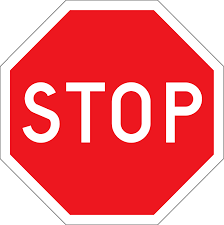
\includegraphics[width =0.3\textwidth]{images/stop}
		\caption{Image of rasterized}
		\label{fig:}
\end{figure}

The image that had to be displayed, was converted into matrix of size 40x40 with each an entry of 12 bits, 3 sets of 4 bit. The 4 bits indicate a duty cycle  for each channel of the RGB diode, thereby will each diode receive three pwm signals, that combined will emit a wanted color from the diode.  \\
Using the encoders , would it be  possible to provide some form of information of the angular position of the LED strips, and thereby which pixels had to be displayed. 

\begin{figure}[H]
		\centering
		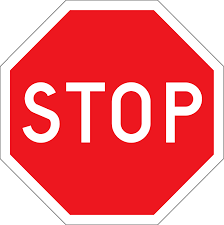
\includegraphics[width =0.3\textwidth]{images/stop}
		\caption{Image rasterized and with the propellor pointing at a certain angle}
		\label{fig:}
\end{figure}
A problem faced here was on how to determine which pixel had to be displayed, in a discrete image description. The problem here is given an angle and a endpoint on how to draw a straight line within these two points, and how to determine the in between pixel positions. \\
Finding the endpoint and angle was pretty easy, the angle was given by the encoders, and the endpoint could easily be calculated trig identities. \\

To draw the line between two points (being the startpoint and the endpoint) were an modified version of Bresenham line algorithm used,  modified as the original algorithm is only capable of handling cases from where the slope between the two points is between 0 and 1. \\

The Bresenham line algorithm is an algorithm used for determining the in between points in raster grid.  It start by computing the change in the x-axis and y-axis  between the start and endpoint, and thereby define a major axis as the one which change with the highest change. 


The major axis is used define the direction which the algorithm should move along. 

\begin{figure}[H]
\center
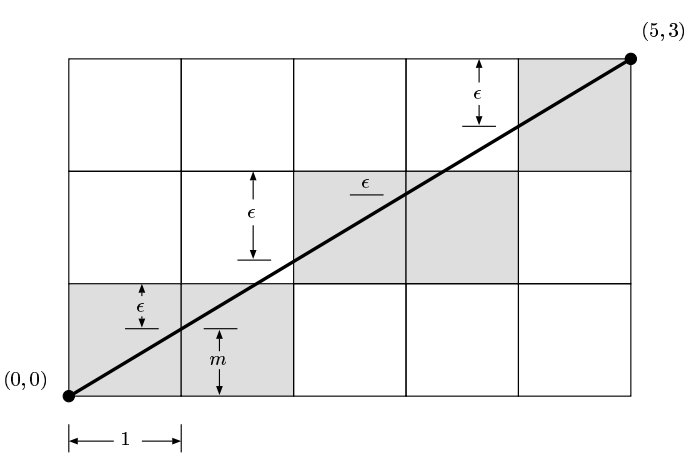
\includegraphics[width = 0.6\textwidth]{images/bresenham}
\caption{Bresenham line algorithm applied on a simple case}
\label{fig:bresenham_line}
\end{figure}
\todo[inline]{http://www.idav.ucdavis.edu/education/GraphicsNotes/Bresenhams-Algorithm.pdf}

in the example given in figure \ref{fig:bresenham_line} the major axis is X. In a main loop will the variable x be incremented by one, and for each incrementation will the y coordinate be incremented with an value $m$ which is defined as $$m = \frac{dy}{dx}$$ while incrementing the y value is an the error bound $\epsilon$  kept which represent the the negative distance between the real line and top edge pixel.  The value is incremented with m for each time the major axis coordinate is incremented by one. \\
$\epsilon$ becomes greater than zero  if the real line has moved upwards according to the previous x value, when it occurs will the y value  be incremented with one, and $\epsilon$ will be recomputed to its new value as 1 - $\epsilon$. \\

As long as the  value  epsilon  is below 0, will the y coordinate only increment in steps of m. 

Using the method would it be possible to output line at the different angles, and thereby display the image when the motors was spinning. 



%This means that everything we see is a subtle blend of what is happening now and what happened a fraction of a second ago.